\documentclass[11pt]{article}

\usepackage[portuguese]{babel}
\usepackage[T1]{fontenc}
\usepackage[utf8]{inputenc}
\usepackage{amsmath}
\usepackage{graphicx}
\usepackage{subfig}
\usepackage[colorinlistoftodos]{todonotes}
\usepackage{listings}
\usepackage{color} 
\usepackage{float}
\usepackage[font={footnotesize}]{caption}
\usepackage{xcolor,colortbl}
\usepackage{array}
\usepackage{fixltx2e}
\setcounter{secnumdepth}{4}


\linespread{1.3}
\usepackage{indentfirst}
\usepackage[top=2cm, bottom=2cm, right=2.5cm, left=2.5cm]{geometry}

\begin{document}
	
\begin{titlepage}
	\begin{center}
		
		\hfill \break
		\hfill \break
		
		
\includegraphics[width=0.3\textwidth]{./logo}~\\[1cm]
		
		\textsc{\Large Mestrado Integrado em Engenharia Electrotécnica e de Computadores}\\[1.5cm]
		\textsc{\huge Sistemas Electrónicos de Processamento de Sinal}\\[0.25cm]
		
		{\huge \bfseries BPSK Modem \\[1.2cm]}
		
		Grupo n.º 2/3 \vspace{0.3cm}
		
		\begin{tabular}{l r}
			André Filipe Barroso Cerqueira \hspace{1mm} & n.º 65144 \\
			Guilherme Branco Teixeira \hspace{1mm} & n.º 70214  \\
			João André Catarino Pereira & n.º 73527
		\end{tabular}
		
		\hfill
		\hfill
		
		segunda-feira 15h30 - 18h30, LE1
		
		\footnote{As linhas de código apresentadas durante o relatório têm como objectivo demonstrar a maneira de raciocinar na resolução de problemas, não representando uma cópia exata do código usado em laboratório, podendo até, serem consideradas \textit{pseudo-código}}
		\vfill
		
		{\large Lisboa, 17 de Abril de 2015} 
		
	\end{center}
\end{titlepage}

\section{Índice}

\section{Introdução}

Este trabalho consiste na primeira parte do projecto de laboratório da cadeira: desenvolvimento de um modem de $Binary$ $Phase$ $Shift$ $Keying$ (BPSK). 

Teve como objectivo a familiarização com o ambiente de desenvolvimento integrado de DSP que consiste nas placas de desenvolvimento DSK TMS320C6416 e DSK TMS320C6713 da $Texas$ $Instruments$ e no software de desenvolvimento $Code Composer Studio v5.5$. Para tal correram-se dois projectos exemplo (sine8\_buf e loop\_intr) e, usando as ferramentas de debug, alteraram-se certos parâmetros de forma a observar os efeitos nos sinais resultantes. Também se consolidaram os conhecimentos adquiridos desenvolvendo dois mini projectos: um oscilador sinusoidal controlado numericamente e o modulador do modem BPSK.

%objectivo do laboratorio
%
%o que foi feito
%
%o q o relatorio vai falar

\section{Projecto}

\subsection{Projectos de Demonstração}
-Resumo das funçoes e os seus objectivos com especial importancia ao loop

-Relaciona-las com as suas utilizaçoes no projecto em si

\subsubsection{sine8\_buf}
\label{sec:sine8}
O objectivo deste projeto é representar a função sinusoidal, multiplicada por um determinado ganho, através de um conjunto de amostras que equivalem a um período da mesma, repetindo nos períodos seguintes esse mesmo conjunto. Este procedimento é realizado através da rotina de interrupção presente no programa. 

Ao analisar o código deste projeto à primeira vista podemos concluir logo que este usa uma frequência de amostragem de 8 kHz , tem um ganho $G=10$ predefinido e usa 8 amostras para representar a sinusoide. Depois de observar a sinusoide no osciloscópio variou-se o ganho a fim de perceber a sua influência e também o seu limite.
 
Para compreender o limite desta sinusoide é necessário ter em conta que se usa o formato de vírgula fixa Q15 para as amostras da sinusoide. Este formato tem como limite o valor $(2^{15}-1) = 32767$. Considerando o valor máximo da sinusoide, se multiplicarmos a mesma por um ganho G=33 obtemos um valor superior ao permitido pelo formato Q15, fazendo com que nesses pontos o valor da sinusoide "caia".     

\subsubsection{loop\_intr}
\label{sec:loop}
Este projeto tem como objectivo fornecer-nos um template para os próximos projetos, em termos de comunicação com a placa e rotina de interrupção. Pode-se observar nas últimas linhas de código como se liga os sinais de entrada e saída aos canais da placa.

(comentario André)No projecto anterior observou-se os efeitos de overflow de uma variável. Neste observam-se os efeitos de aliasing(ou não, não me recordo se o DSP tem um filtro anti-aliasing à entrada)  devido ao sinal de line-in ter a mesma frequência que a frequência de amostragem. Se havia anti-aliasing, a partir dos 4khz deixariamos de ver uma sinusoide com os 3.3V. Não fizemos a experiência de mudar para sinal quadrado e variar a frequência, mas provavelmente nao iamos ver um sinal quadrado pois o espectro (infinito) deste teria que ser filtrado pelo anti-aliasing filter.

Vale a pena ir ao lab tirar esta foto?
Resultados do loop??

\subsection{BPSK}

 Demonstração dos Resultados usando como etapas as varias perguntas do enunciado, complementar com as fotos e possiveis tabelas ou partes de codigo

\subsubsection{P1. Oscilador controlado numericamente}

Usando o projecto descrito na secção \ref{sec:loop} como base para a construção de um oscilador controlado numericamente (\textit{NCO}). Um \textit{NCO} é um gerador de sinal digital que cria uma forma de onda discretamente representada no tempo e na amplitude. O nosso \textit{NCO} terá as seguintes características:

\begin{table}[H]
	\centering
	\caption{Características do \textit{NCO} a construir.}
	\label{tab:NCO-car}
\begin{tabular}[c]{|l||c|c|}
	\hline \textbf{Parâmetro} & \textbf{Símbolo} & \textbf{Valor} \\ 
	\hline Freqência de amostragem & $ f_{s} $ & $ 16 kHz $ \\ 
	\hline Frequência mínima & $ f_{min} $ & $ 2 kHz $ \\ 
	\hline Frquência máxima & $ f_{max} $ & $ 6 kHz $ \\ 
	\hline
\end{tabular}
\end{table}

O projecto de contruir o \textit{NCO} seguiu os seguintes passos que estão posteriormente desmitigados:

\begin{enumerate}
	\item Oscilador de Relaxamento (Integrador de Rampa). Secção \ref{para:P1-1}.
	\item Look-up-table (LUT). Parágrafo \ref{para:P1-2}.
	\item Obter sinal de seno através da LUT. Secção \ref{para:P1-3}.
	\item Criação de duas variáveis para controlar a frequência e amplitude. Secção \ref{para:P1-4}.
	\item Variar a frequência do sinal criado com a amplitude do sinal de entrada. Secção \ref{para:P1-5}.
	\item Testar os oscilador com uma sinal de uma onda quadrada à entrada.  Secção \ref{para:P1-6}.
	\item Melhorar qualidade do oscilador com interpolação linear.  Secção \ref{para:P1-7}.
	\item Comparar os espectros.  Secção \ref{para:P1-8}.
\end{enumerate}

\paragraph{P1-1}\label{para:P1-1}

Como referido na secção \ref{sec:sine8}, quando representamos sinais sob o formato de vírgula-fixa Q15 teremos como valor máximo do sinal: $32767$. Como a placa usada no laboratório (DSK TMS320C6713), tem como amplitude máxima na saída de $1 V$, foi usado o formato Q15 para representar o sinal de saída, visto que um sinal representado em Q15 terá amplitude máxima de $ 1-2^{-15} => 32767 $.

Para construir um Oscilador de Relaxamento foi criado um programa que aumentasse constantemente o sinal à saída de modo a que este tivesse um aspecto de rampa. O incremento teria de tomar um valor, tal que $32767$ fosse seu múltiplo. Ao verificar a tabela \ref{tab:NCO-car}, podemos chegar aos seguintes valores de incremento com as suas frequências correspondentes:


\begin{table}[H]
	\centering
	\caption{Valores a atribuir ao incremento do sinal na saída.}
	\label{tab:incrementos}
	\begin{tabular}[c]{|l||c|}
		\hline \textbf{Frequência de saída($f_0$)} & \textbf{Incremento($\Delta$)}\\ 
		\hline $ 2 kHz \quad (f_{min}) $ & $ 8192 $\\ 
		\hline $ 4 kHz $ & $ 16384 $  \\ 
		\hline $ 6 kHz \quad (f_{max}) $ & $ 24576 $ \\ 
		\hline
	\end{tabular}
\end{table}

Os valores calculados na tabela \ref{tab:incrementos} foram calculados através da seguinte fórmula:

\begin{equation}
 f_{0}= \frac{\Delta}{2A}f_{s} \Leftrightarrow \Delta= 2A\frac{f_{0}}{f_{s}} \hspace{3 mm}, A=32767
\end{equation}

Foi então possível obter as seguintes rampas com diferentes frequências:


\begin{figure}[H]
	\centering
	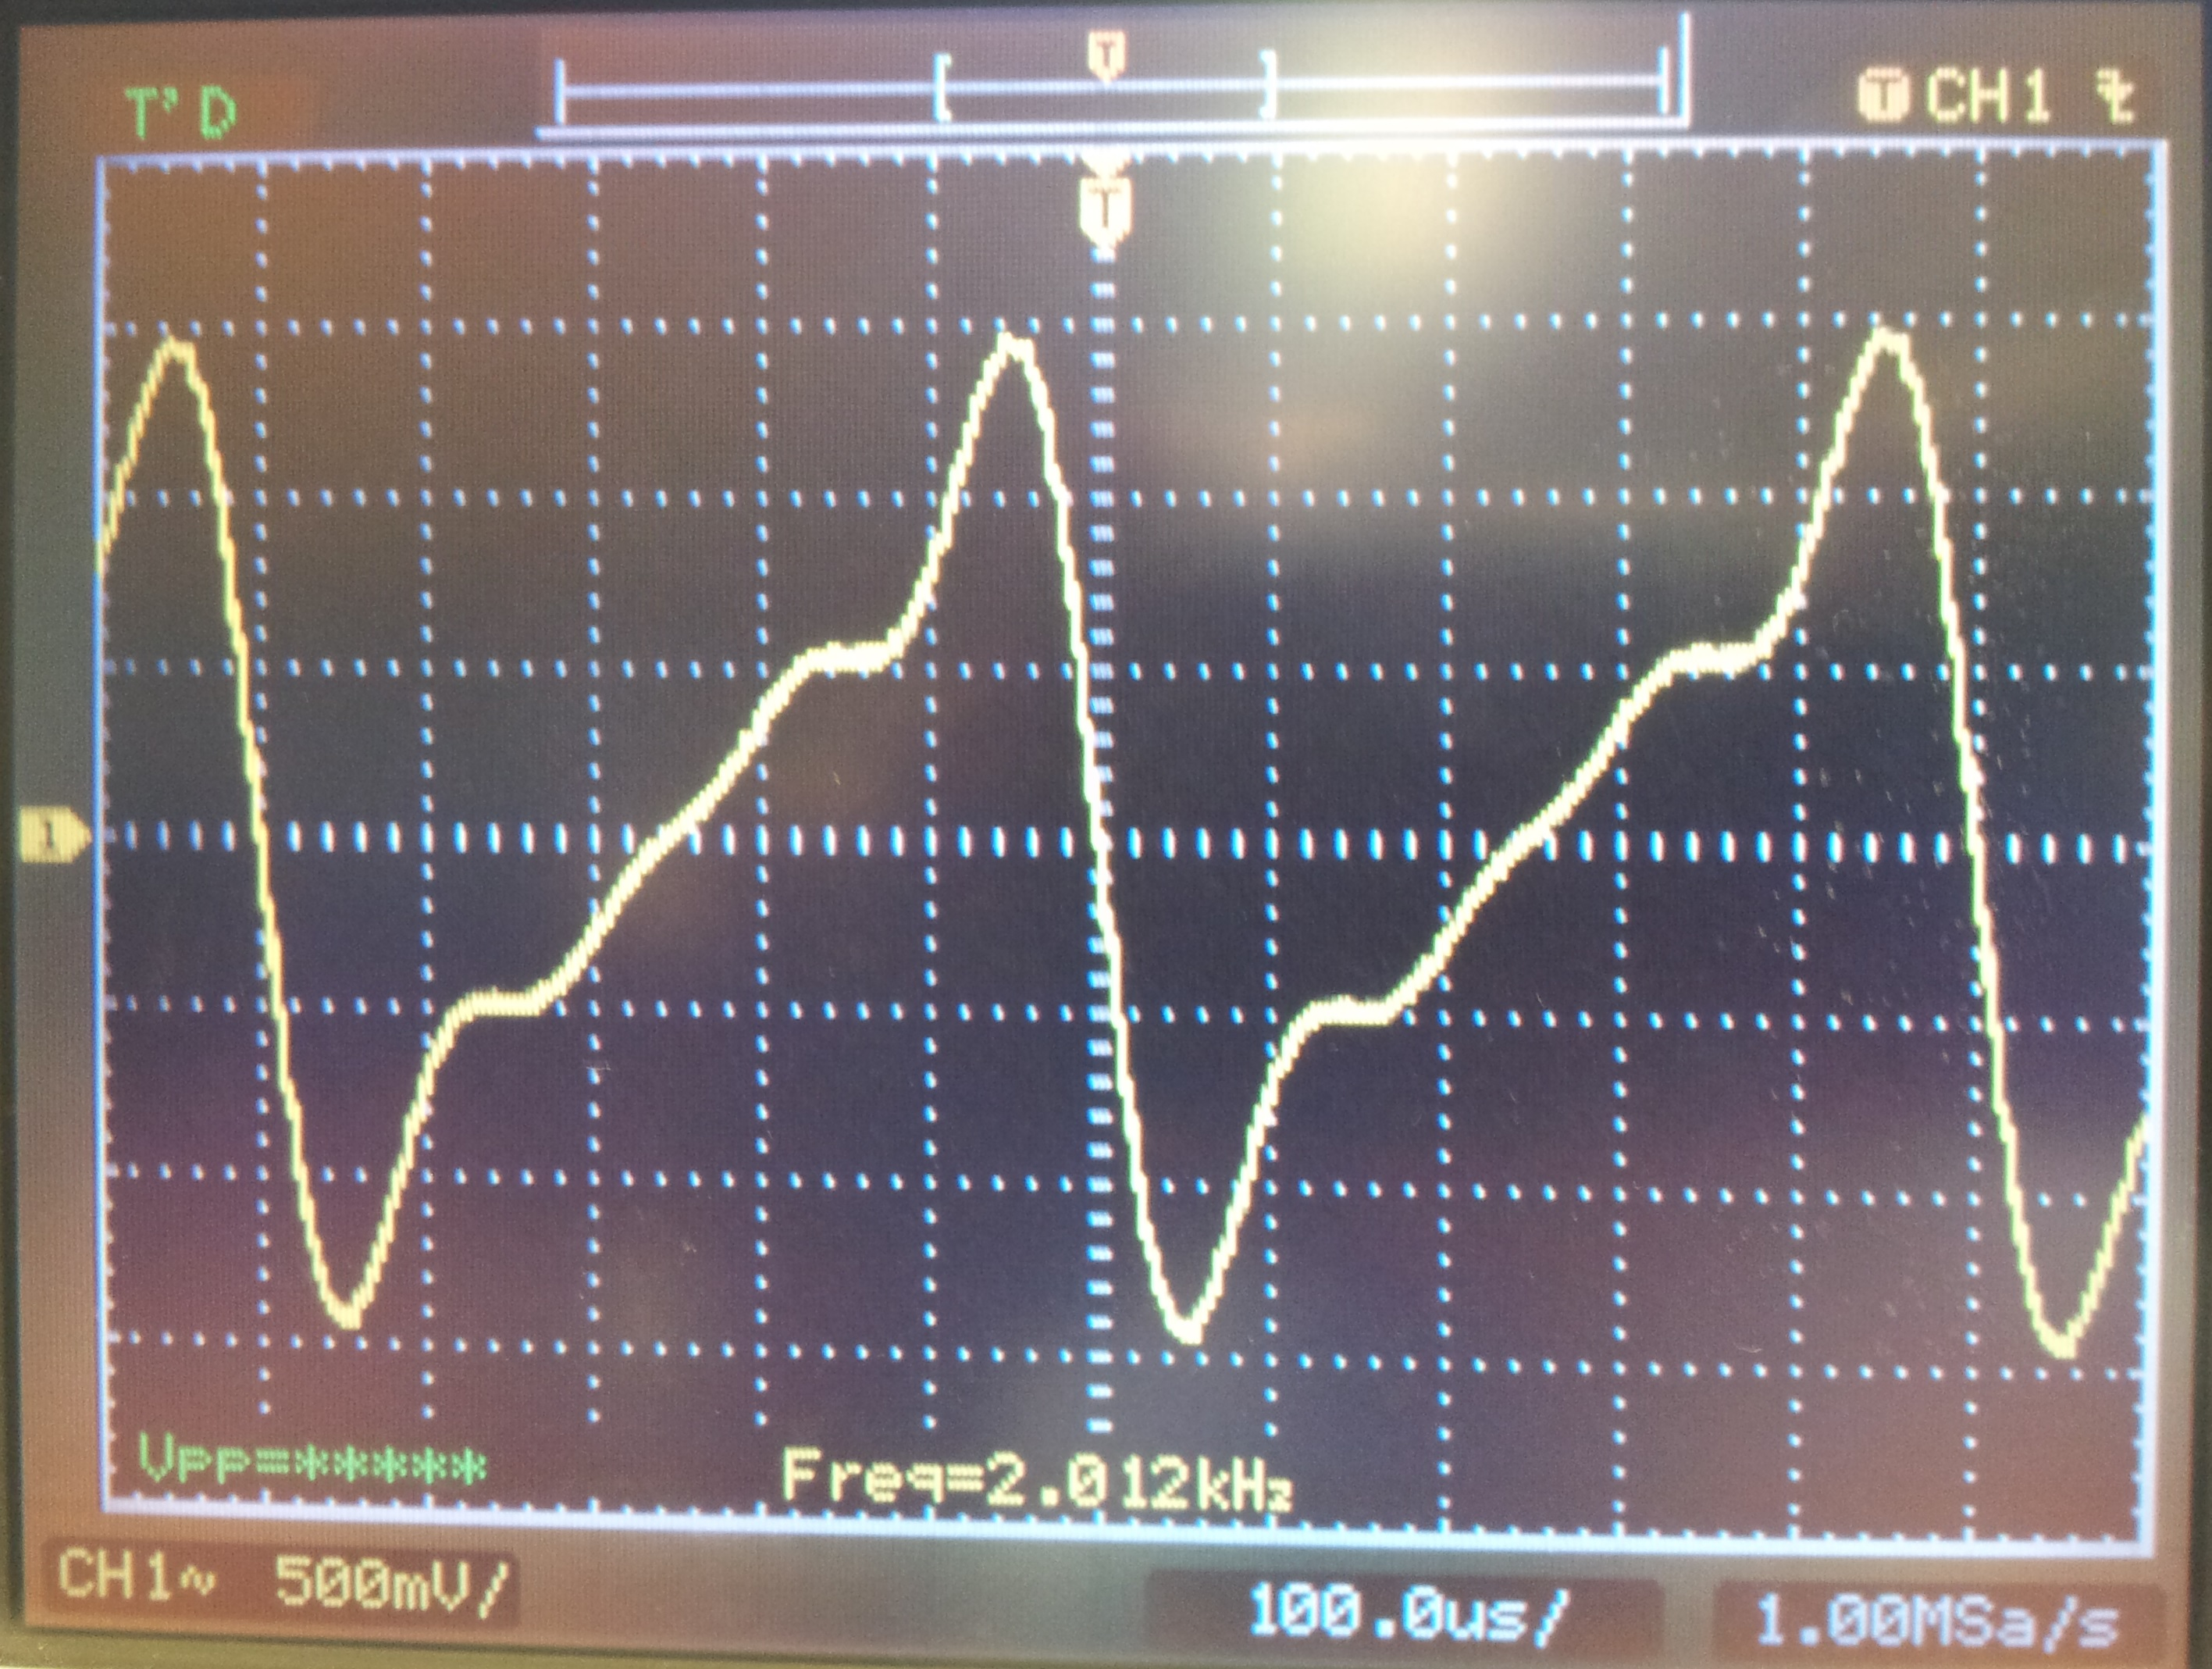
\includegraphics[width=0.5\textwidth]{./P1_2kHz}~\\
	\caption{Rampa com frequência de $ 2 kHz $}
\end{figure}


\begin{figure}[H]
	\centering
	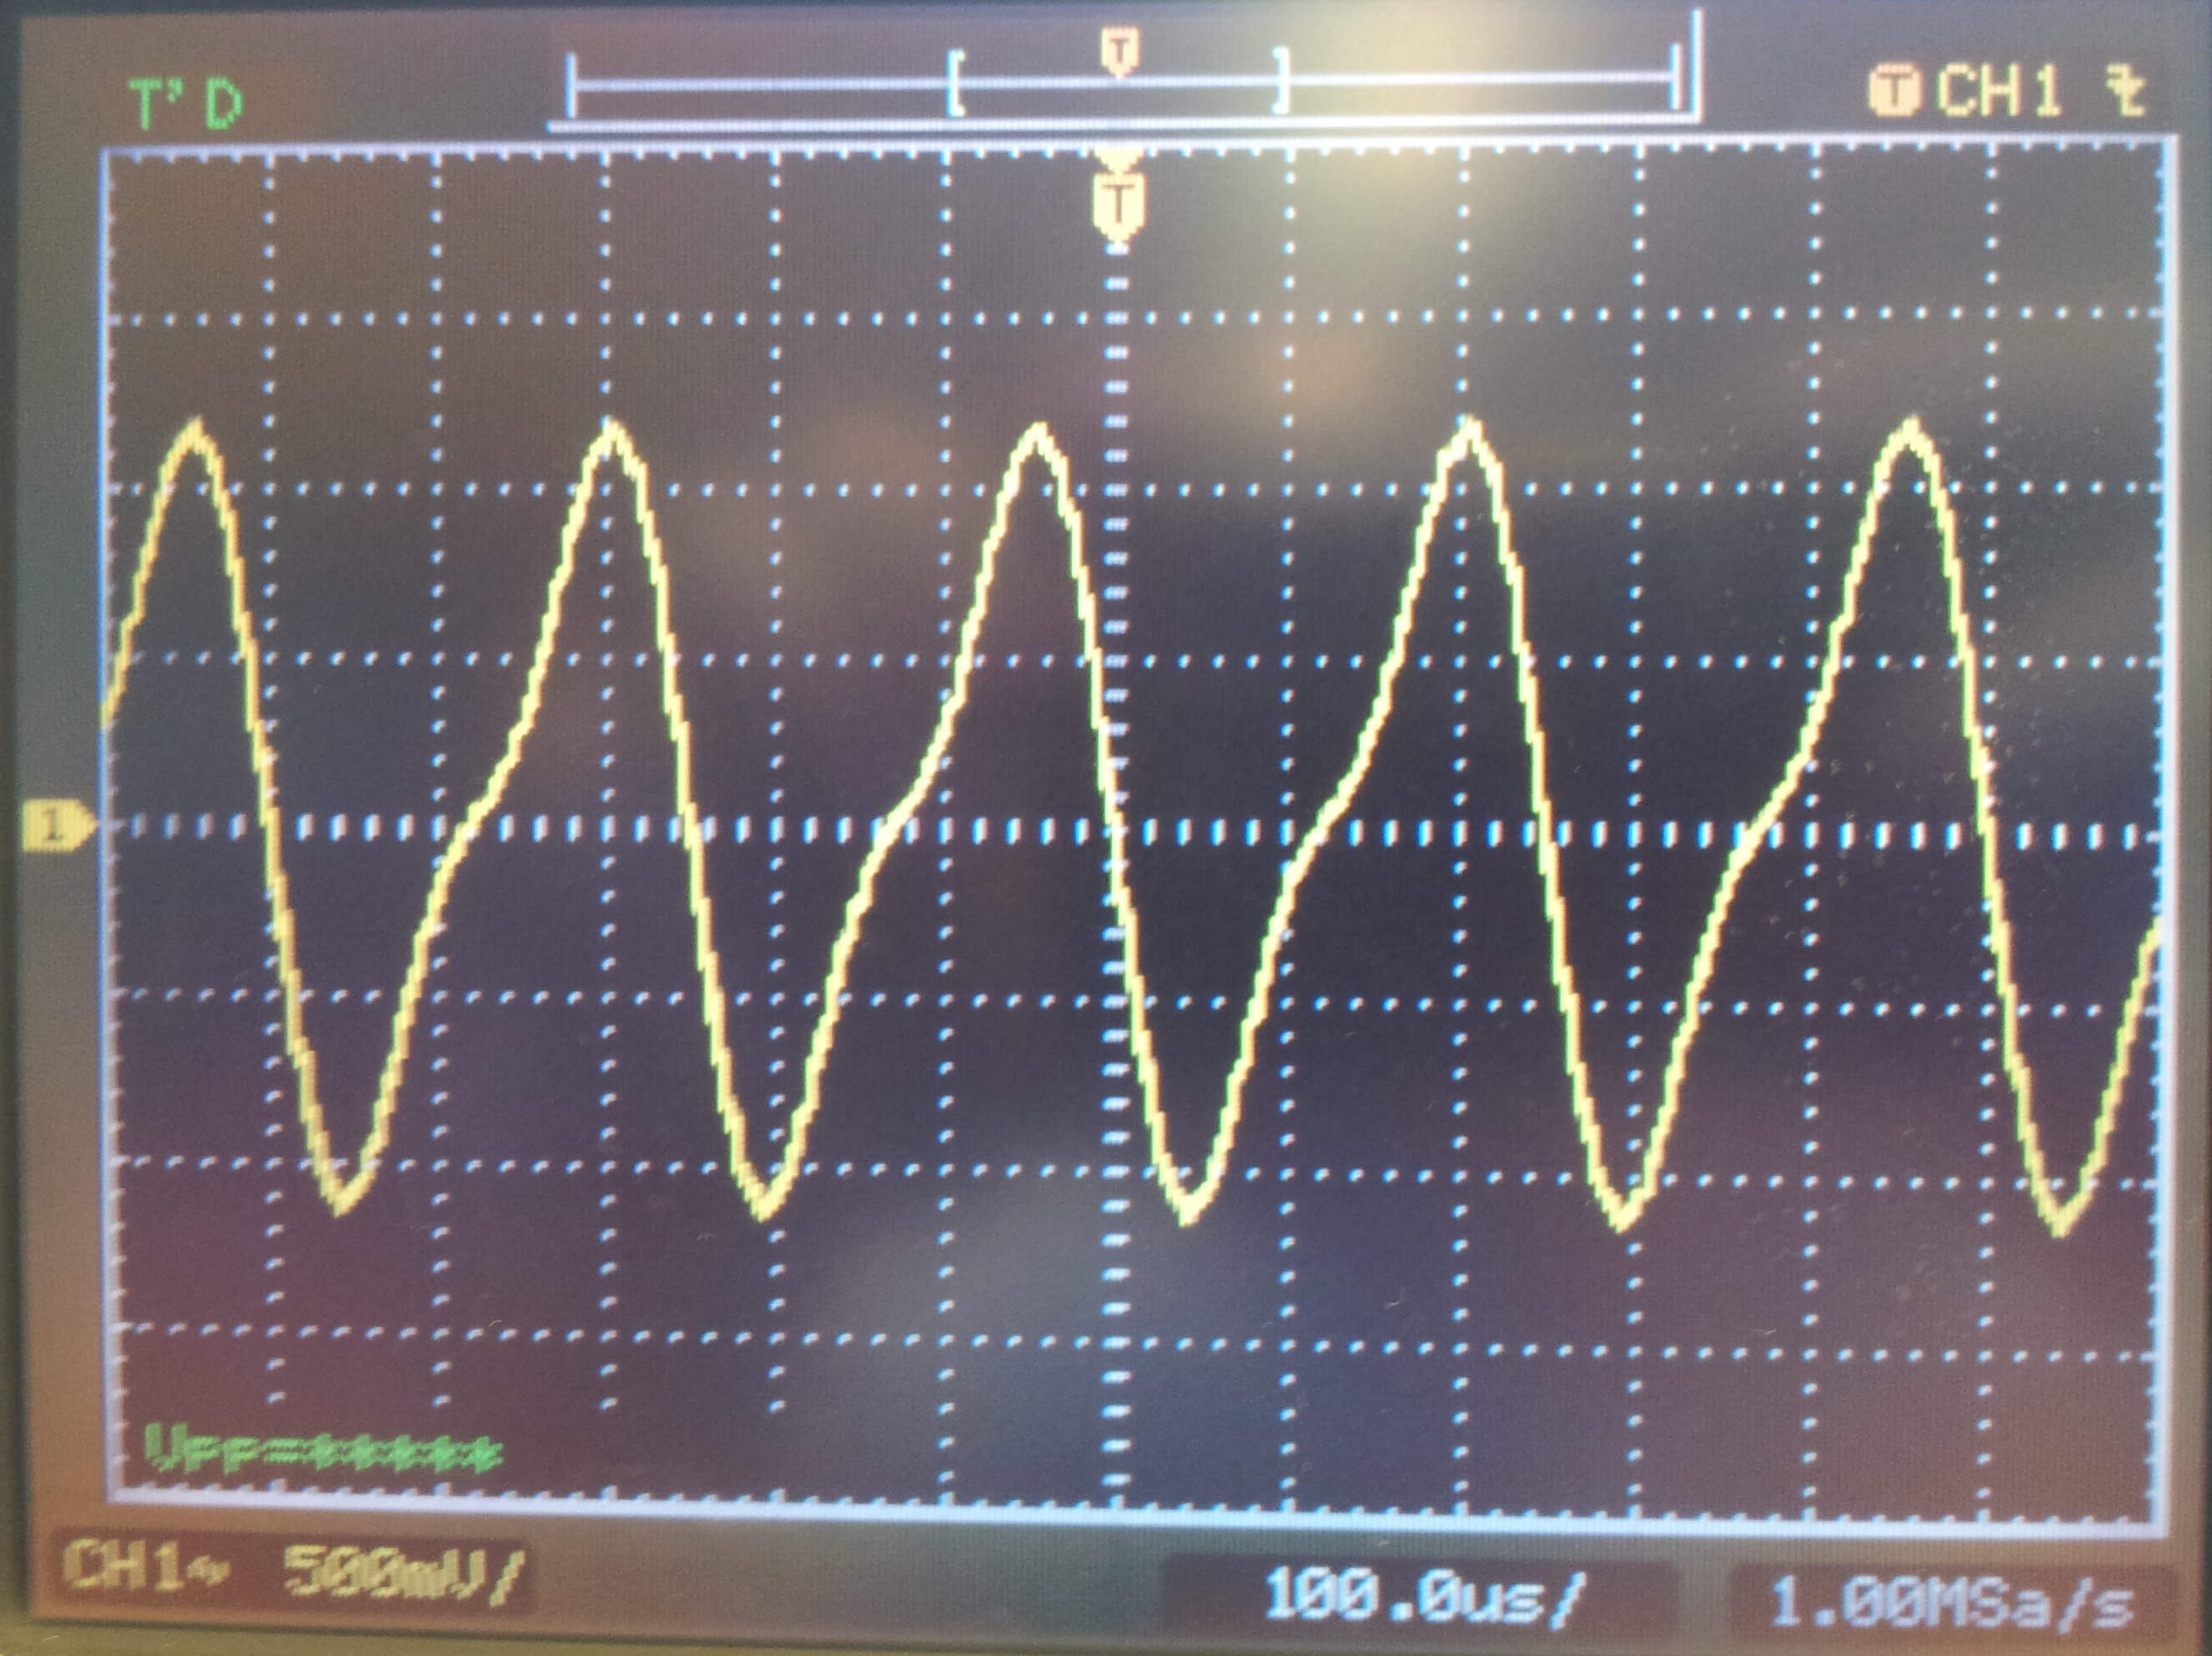
\includegraphics[width=0.5\textwidth]{./P1_4kHz}~\\
	\caption{Rampa com frequência de $ 4 kHz $}
\end{figure}

\paragraph{P1-2}
\label{para:P1-2}

Foi criada uma tabela (LUT) com os valores de meio ciclo de um seno de modo a que seja possível ir retirar os seus valores para criar um sinal sinusoidal. Esta tabela teria 32 valores e foi construída pela seguinte equação:

\begin{equation}
32767*\sin \dfrac{n \pi}{32},  \quad \quad n=0,1,2,...,31
\end{equation}

\paragraph{P1-3}
\label{para:P1-3}

Usando como base as rampas criadas na secção \ref{para:P1-1} como método de indexação, foi possível criar um sinal de uma sinusóide através da tabela de LUT criada na secção \ref{para:P1-2}.

Para a indexação são usados os 5 bits mais significativos (excluindo o bit de sinal) do sinal da rampa, esses 5 bits irão indexar e escolher qual o valor da tabela de LUT a usar para criar a sinosóide. Este processo foi efectuado com o seguinte pedaço de código dentro do ciclo:

\begin{lstlisting}
	rampa=rampa+incremento;    //Criar a rampa
	index=rampa>>10;
	index=31 & index;         //Usar apenas 5 bits
	sinusoide=LUT[index];
\end{lstlisting}

O resultado foi o que se pode observar na seguinte figura:

\begin{figure}[H]
	\centering
	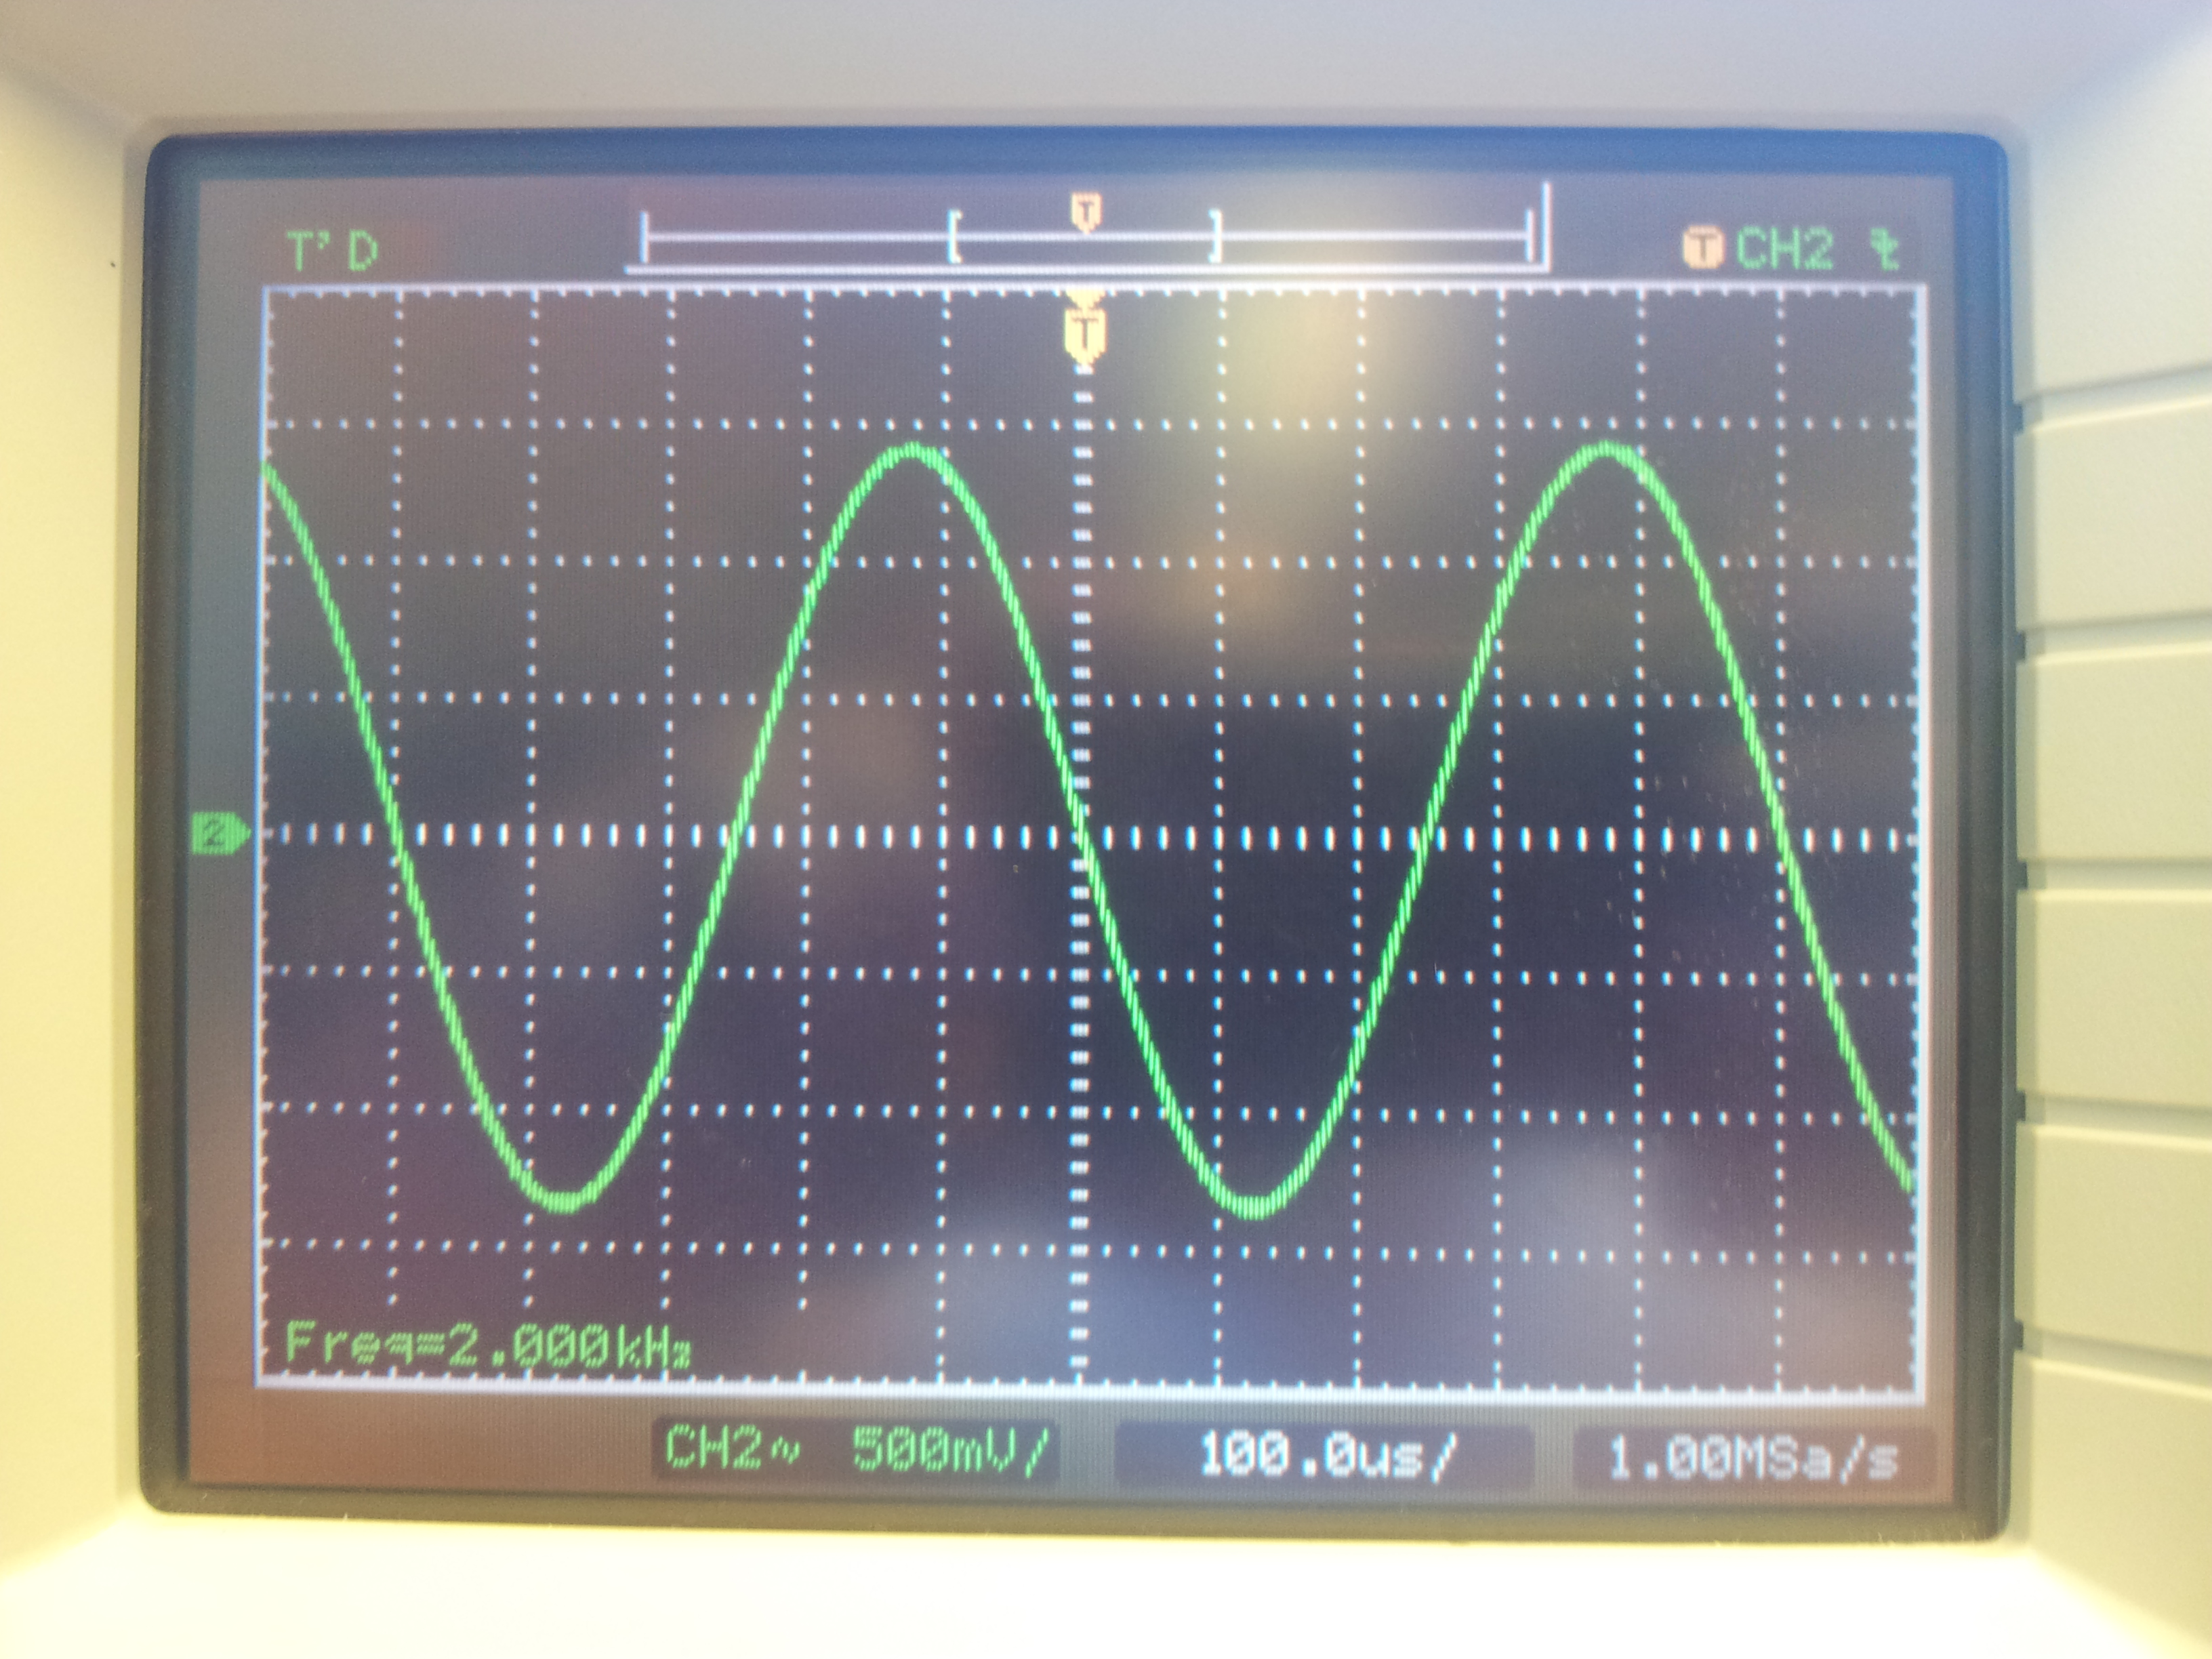
\includegraphics[width=0.5\textwidth]{./P1_1seno}~\\
	\caption{Sinal sinusóide criado de $ 2 kHz $.}
\end{figure}

Como se pode observar na figura foi possível criar um sinal sinusóide usando uma rampa e uma tabela com valores de seno.

\paragraph{P1-4}
\label{para:P1-4}

Foram criadas duas variáveis para fosse possível controlar a frequência e a amplitude do sinal à saída, \textit{incremento} e \textit{amplitude}, respectivamente.

A primeira variável foi já antes referida, nas secções \ref{para:P1-1} e \ref{para:P1-3}. Esta variável, caso alterada iria alterar a frequência da rampa, e por consequência, a frequência do sinal de saída. Como se pode observar na tabela \ref{tab:incrementos}, esta variável terá como limite máximo o valor $ 24576 $ e como limite mínimo $ 8192 $. Podemos também concluir que quanto maior for esta variável, maior a frequência do sinal de saída, tal como se o seu valor diminuir, a frequência de saída irá diminuir também.

A segunda variável (\textit{amplitude}) foi criada com o propósito de modelar a amplitude do sinal de saída, esta causou mudanças mais significativas no código, tal como se pode verificar:

\begin{lstlisting}
	rampa=rampa+incremento;
	index=rampa>>10;
	index=31 & index;        
	aux=amplitude*LUT[index];
	aux=aux<<1;            //Retirar bit de sinal extra
	sinusoide=-aux>>16;    //Colocar a variavel com 16 bits em Q15
\end{lstlisting}

Esta variável tem como valor máximo $ 32767 $, pois os valores afixados na tabela LUT já apresentam um valor com a amplitude máxima de Q15, não tendo assim problemas em relação ao formato de representação nem à amplitude do sinal transmitido à placa.

Deste modo foi possível ter duas variáveis, \textit{incremento} e \textit{amplitude}, que modelavam a frequência e a amplitude do sinal de saída respectivamente.

\paragraph{P1-5}
\label{para:P1-5}

Para que a frequência do sinal de saída seja modelado através da amplitude do sinal de entrada, o sinal de entrada terá de controlar a variável \textit{incremento}.

Um exemplo de garantir que isto era possível era receber um novo valor para a variável \textit{incremento}, sendo que este valor vinha diretamente da entrada:

\begin{lstlisting}
	incremento=-inbuf;
	rampa=rampa+incremento;
	(...)
\end{lstlisting}

Deste modo, quando se aumentava a amplitude do sinal de entrada, a variável \textit{incremento} aumentava, e por consequência também aumentava a frequência de entrada.

\paragraph{P1-6}
\label{para:P1-6}

\paragraph{P1-7}
\label{para:P1-7}

Com o objectivo de melhorar a qualidade do sinal criado vai ser usado o método de interpolação linear descrito na seguinte equação:

\begin{equation}
y=y_{1}+(y_{2}-y_{1})*\delta_{x}
\end{equation}

Sendo que $ \delta_{x} $ refere-se aos 10 bits menos significativos ignorados na altura em que se retira o valor \textit{index} com o propósito de indexação. O processo de recolher o valor de $ \delta_{x} $ e do cálculo da interpolação estão descrito nas seguintes linhas de código:

\begin{lstlisting}
	rampa=rampa+delta;
	deltaX=1023 & rampa;   //Retirar os 10 bits menos significativos
	deltaX=deltaX<<5;      //Representar deltax em Q15
	index=rampa>>10;
	index=31 & index; 
	aux=amplitude*LUT[index];
	aux=aux<<1;
	sinusoide=-aux>>16;
	Y1=sinusoide;
	aux=amplitude*LUT[index+1];
	aux=aux<<1;
	Y2=-aux>>16;
	aux=(Y2-Y1)*deltaX;
	aux=aux<<1;
	Y=Y1+(aux>>16);
\end{lstlisting}

Sendo que o sinal \textit{Y} corresponde ao sinal com maior qualidade, ou seja, interpolado, e que o sinal \textit{sinusoide} corresponde ao sinal com menor qualidade.

Ambos os sinais podem ser observados na imagem \ref{fig:interp}, embora a sua comparação não poderá ser efetuada na sua observação.


\begin{figure}[H]
	\centering
	\label{fig:interp}
	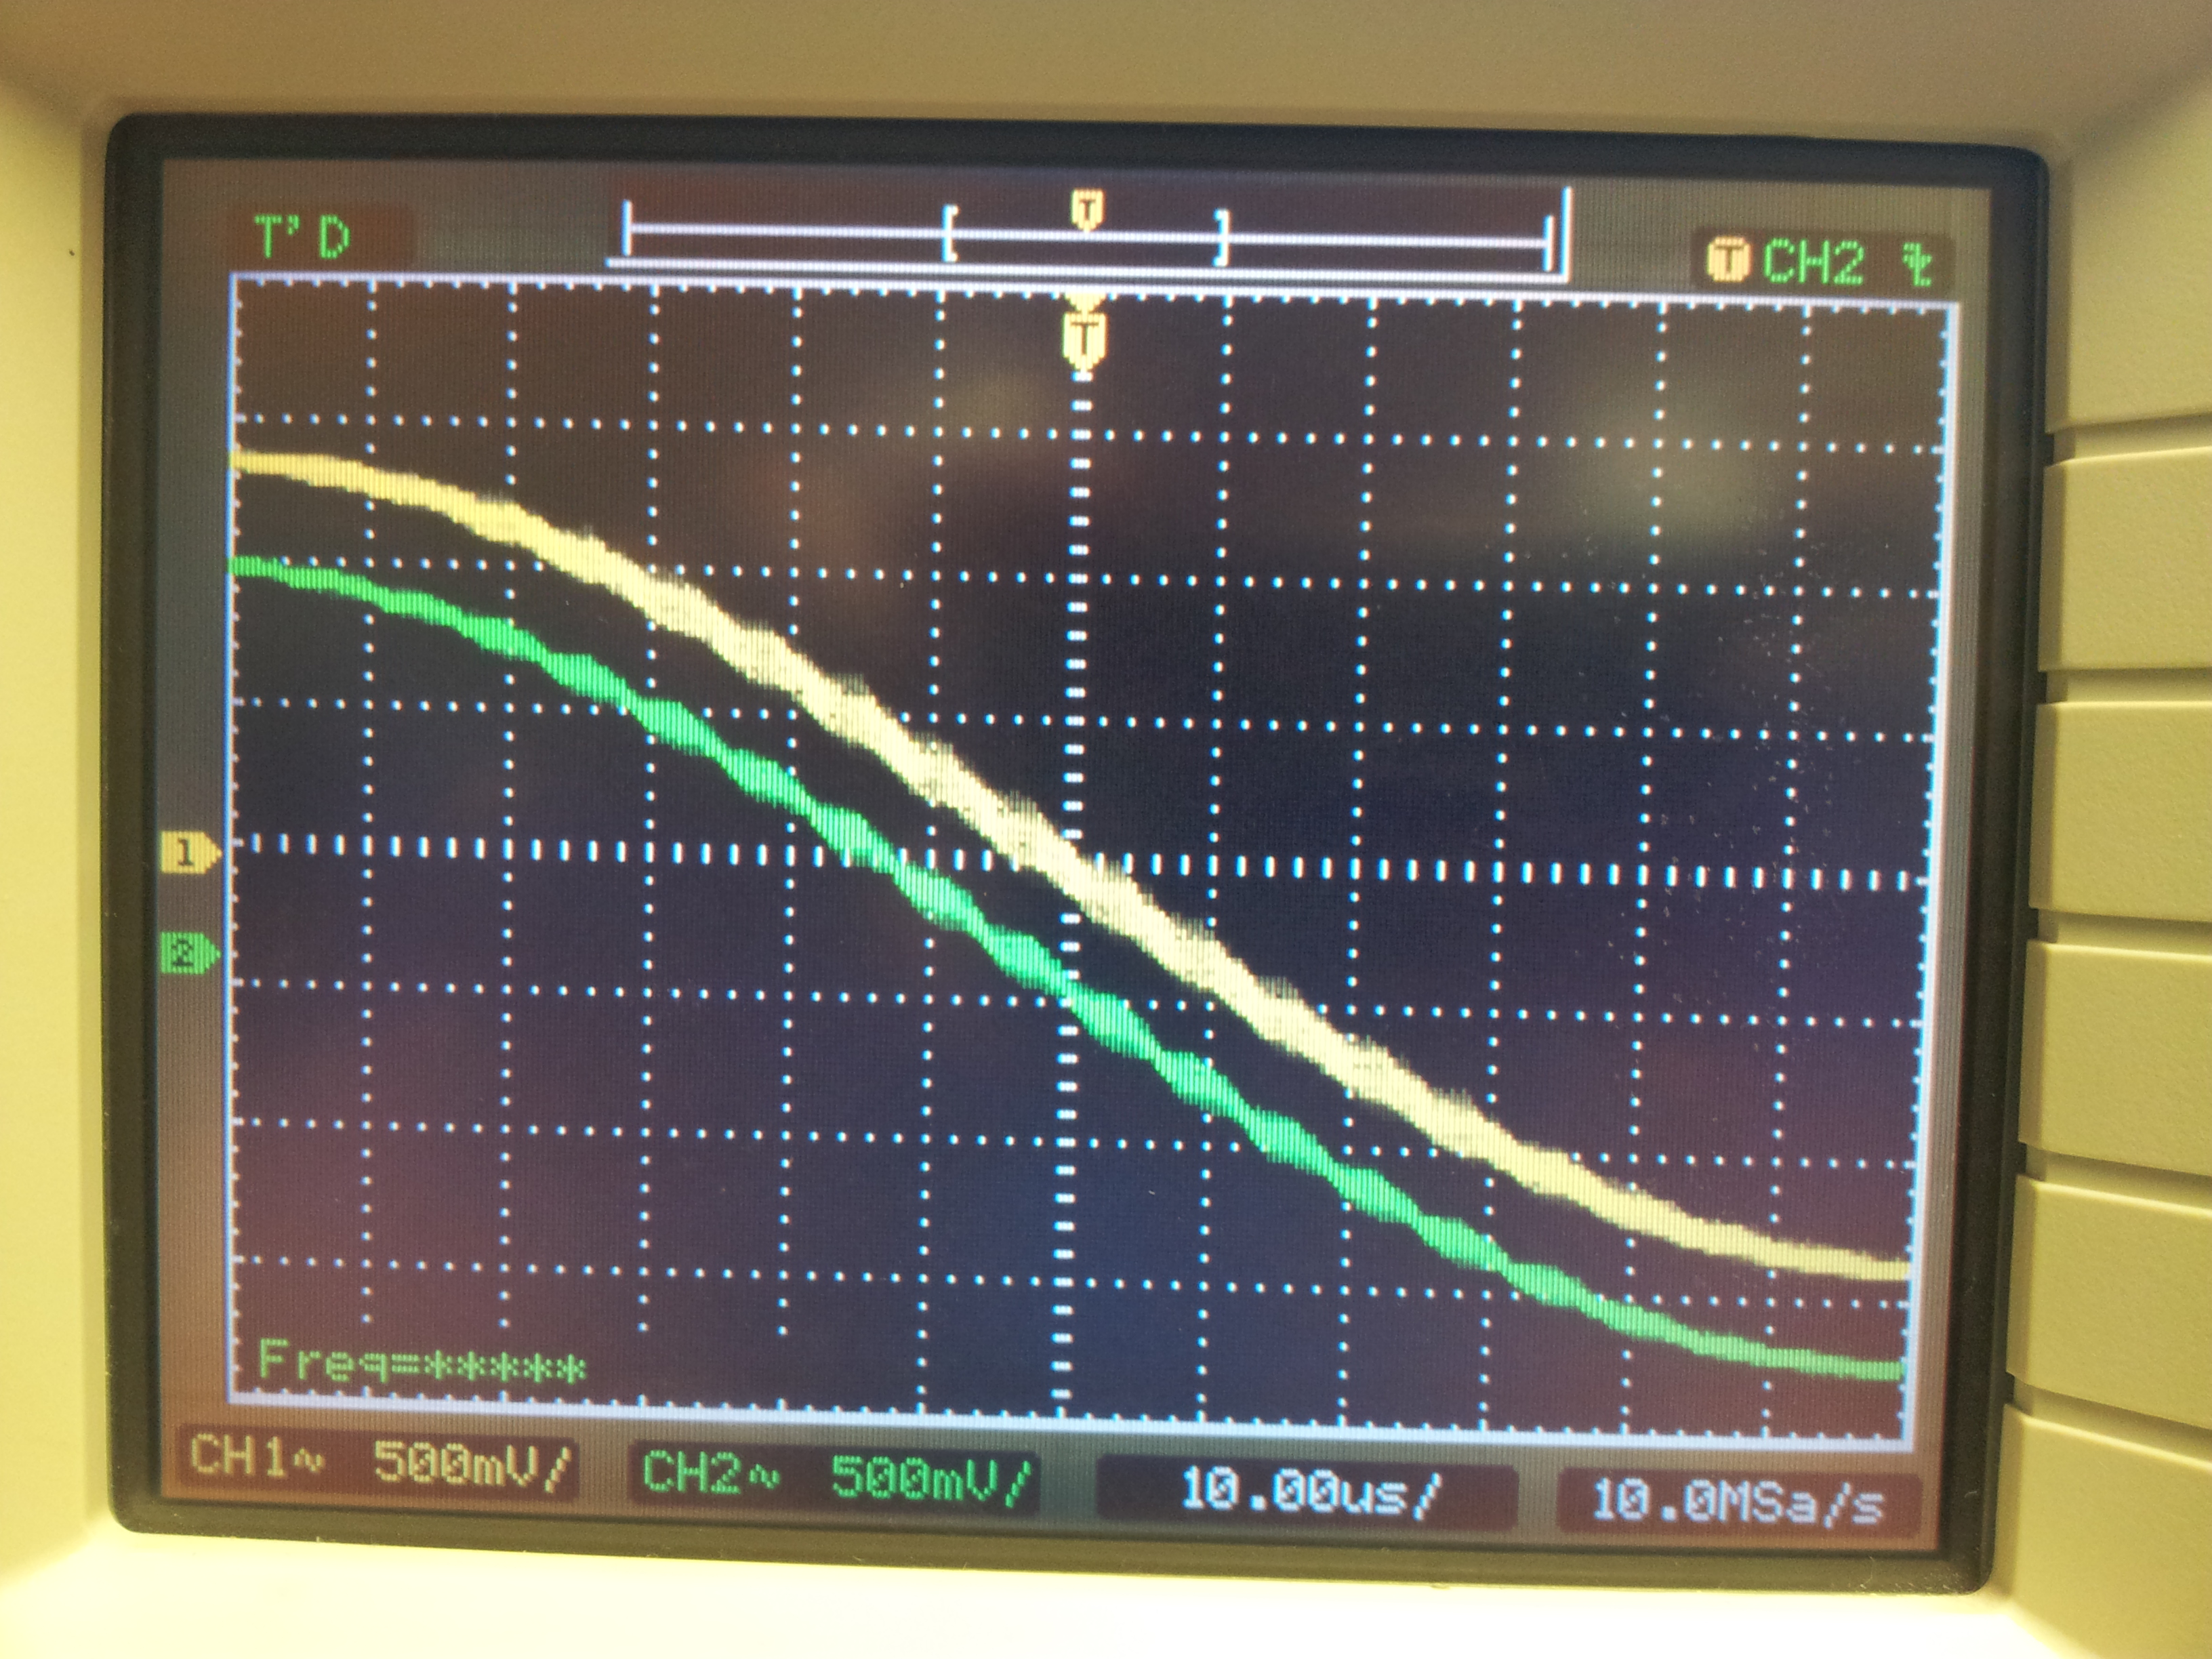
\includegraphics[width=0.5\textwidth]{./P1_interp}~\\
	\caption{Sinal sinusoide com interpolação e sem interpolação.}
\end{figure}

\paragraph{P1-8}
\label{para:P1-8}
%fazer espectros e comparar!!!

\subsubsection{P2. Transmissor BPSK}

%Introdução Teórica
O objectivo deste projeto é criar um transmissor BPSK com recurso a três elementos principais, uma fonte de bits, um codificador diferencial e mapeador, e um modulador.
Neste projeto foi utilizada uma frequência de amostragem $f_s=16$ kHz e uma frequência portadora $f_0=4$ kHz.
%COMPLEMENTAR com alguma teoria
\vfill
%Pergunta 1
Para ter uma fonte de bits no transmissor usa-se um "bit-rate clock" cuja função vai ser criar uma sequência de bits $ b_n $ com $f_b=1$ kbps. Isto significa que, considerando $f_s$, a cada 16 ciclos é gerado um novo bit, alternado em relação ao anterior. Assim, implementou-se um contador que é incrementado em cada ciclo  e que tem uma condição para verificar quando chegar ao valor 16. Ao entrar nessa condição é implementada a lógica para cálculo do novo bit da sequência e o contador é reiniciado.

Para calcular o novo bit, basta negar o bit anteriormente obtido para obter uma sequência de bits alternada, tendo sido concretizado através de uma simples XOR:
\begin{equation}
b_n=b_{n-1} \oplus 1
\end{equation}

Após obter a fonte de bits passou-se ao segundo elemento do transmissor: o codificador diferencial e mapeador. Começando pelo codificador diferencial, este utiliza $b_n$ para aplicar a seguinte operação lógica:
\begin{equation}
c_n=c_{n-1} \oplus b_n
\end{equation}
Assim, com $c_0$ inicializado a zero codifica-se a sequência de bits $ b_n $. Ao gerar $ b_n $ e $ c_n $ obtém-se dois sinais que variam entre "0" e "1" só que $ c_n $ tem o dobro do período (figura X).

IMAGEM bn com cn
\vfill
%\begin{figure}[h]
%	\centering
%	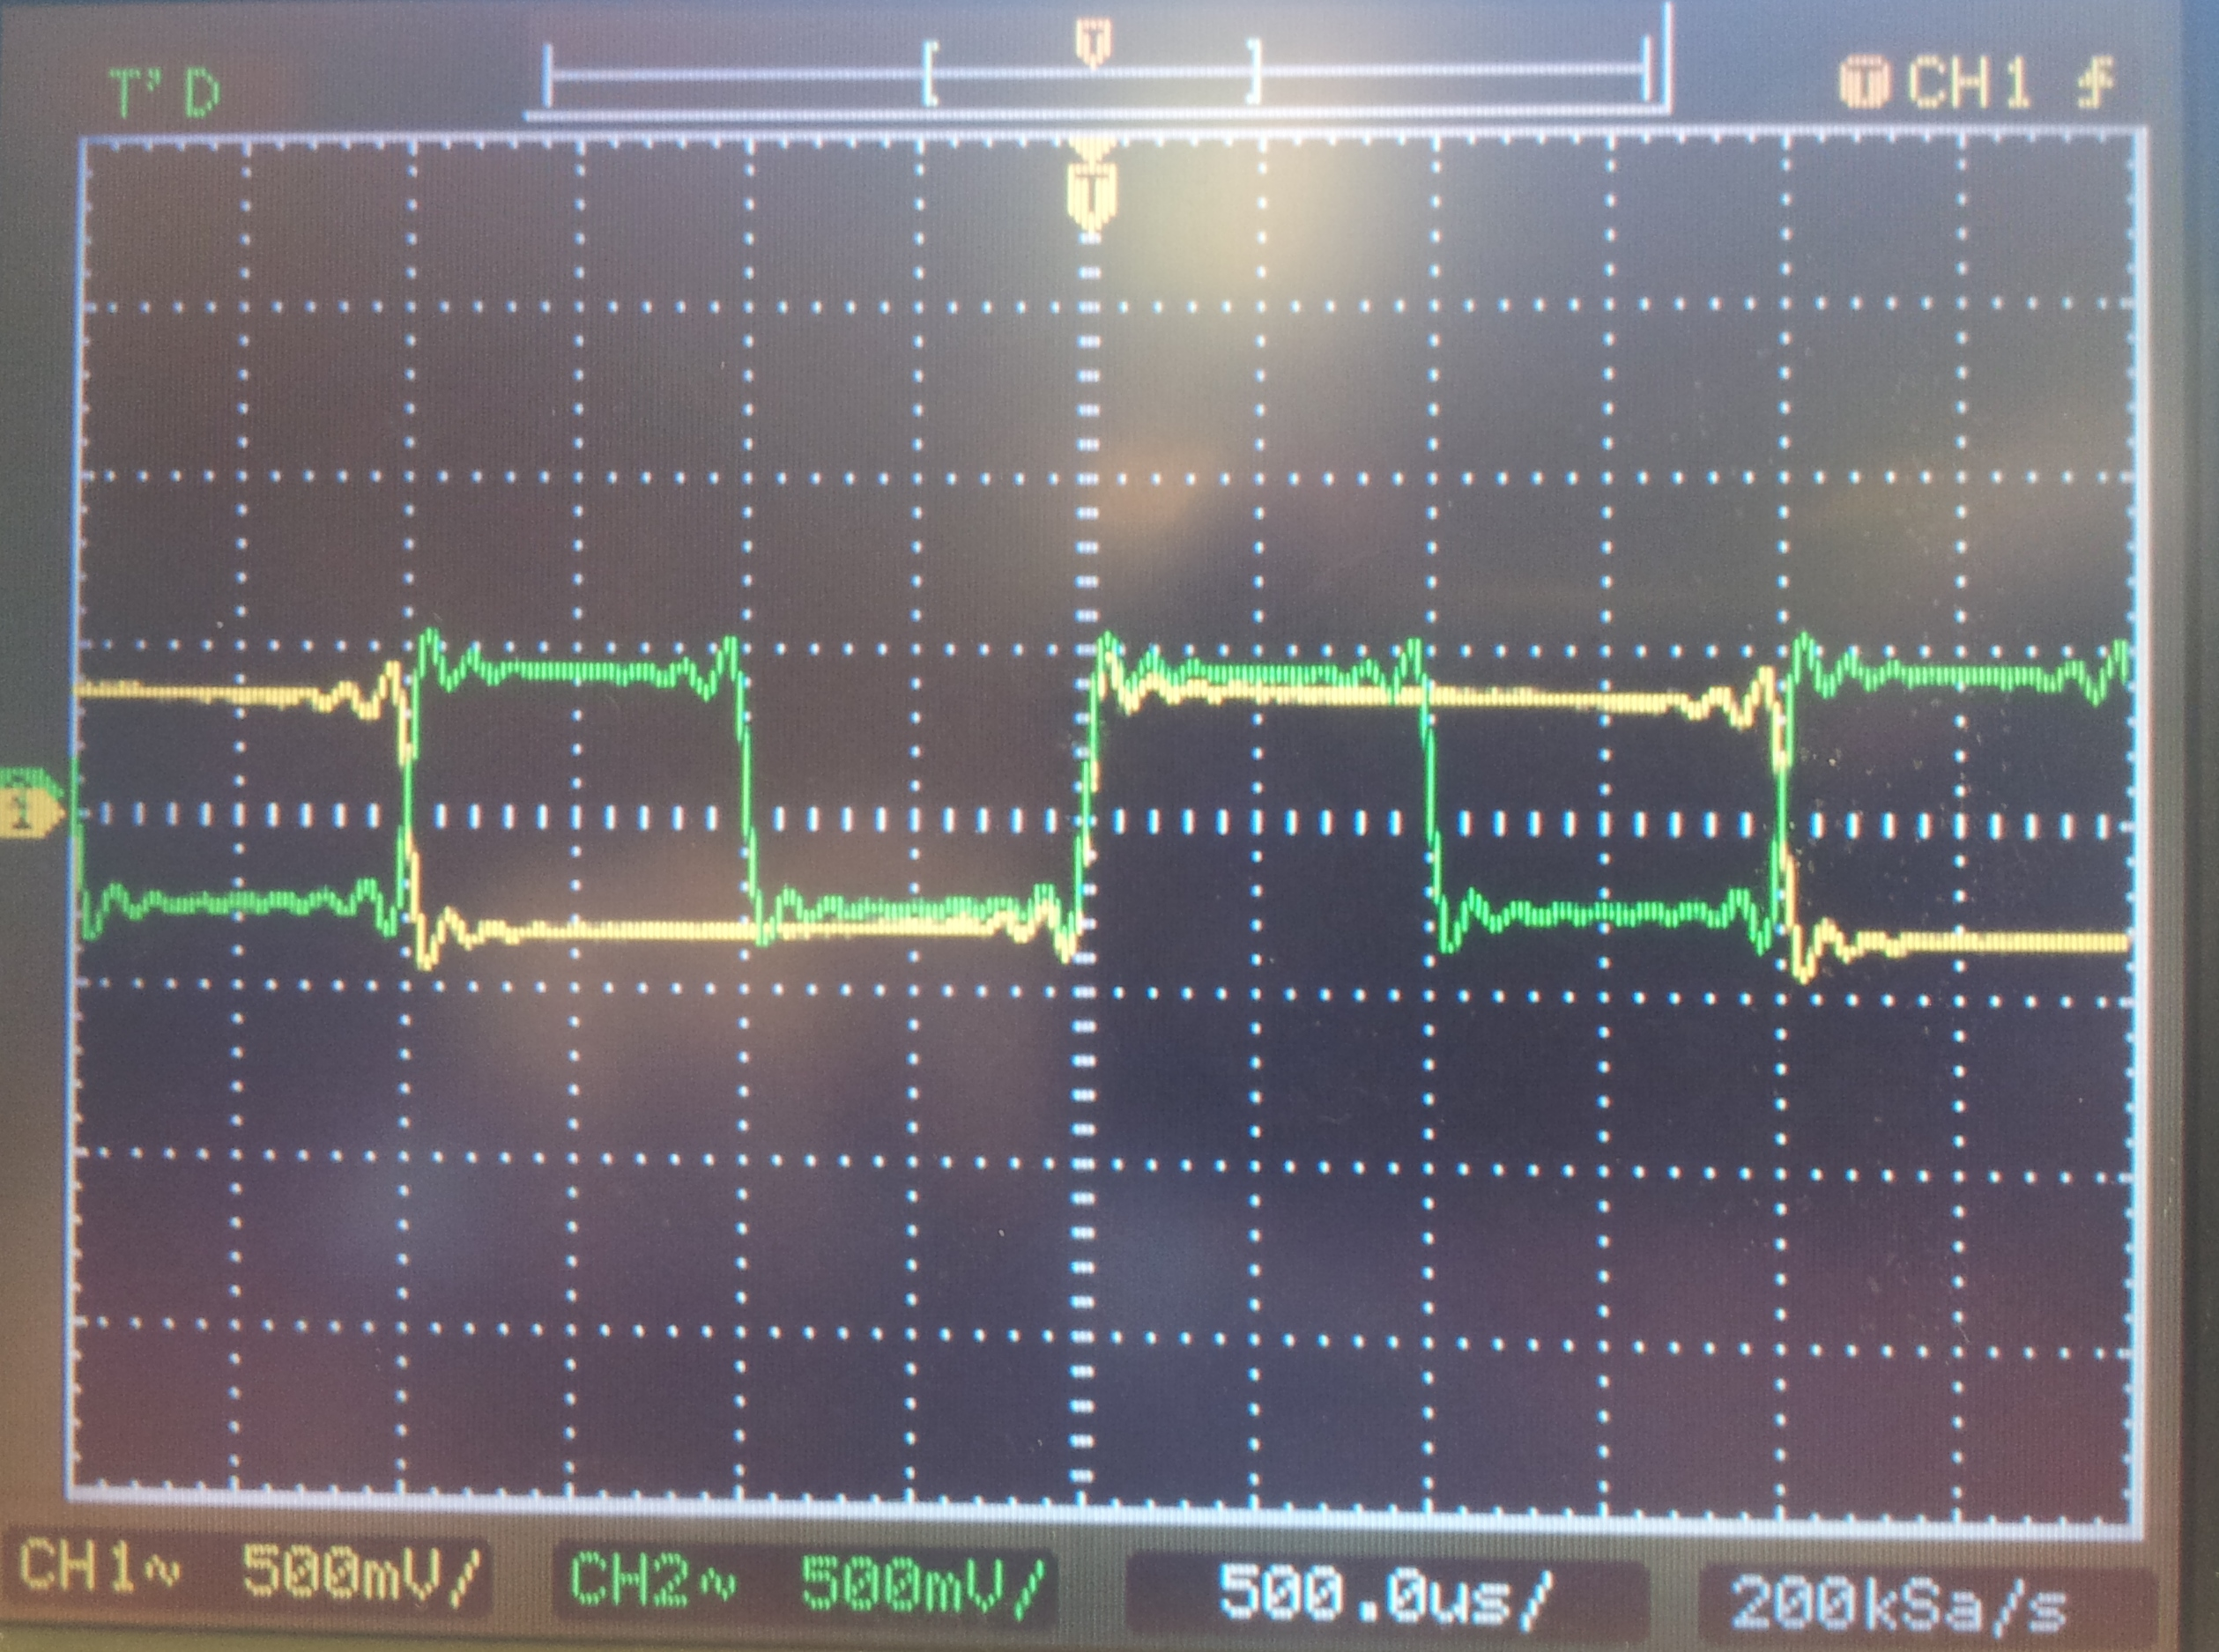
\includegraphics[width=0.5\textwidth]{./bn_cn}~\\
%	\caption{$ b_n $(verde) e $ c_n $(amarelo)}
%\end{figure}

%\vspace{-0.4cm} %este espaçamento dá cabo da formatação toda no meu tex.
Depois de obter $ c_n $ passa-se ao mapeamento do mesmo,
%explicar f=500Hz => uma vez que uma sequencia alternada de bits é o mesmo que uma onda quadrada, divide-se o bit rate 1kbps por dois pois cada meio ciclo da onda quadrada corresponde a um bit.
%complementar com o que?

%Pergunta 2
Falta agora gerar a onda portadora a modular. Esta foi implementada de forma mais simples face ao projeto anterior uma vez que a frequência é estática (4 kHz) e este valor consiste numa fração inteira da frequência de amostragem (16kHz).
Em primeiro lugar criou-se uma tabela com quatro valores dum período da sinusoide, sendo esta: %fazer tabela com valores

Escolheram-se estes valores uma vez que o período de amostragem coincide com os instantes de máximo, mínimo e zero-crossing da portadora. Para gerar a portadora recorreu-se a um contador que, em cada interrupção (ocorrendo em cada instante de amostragem, como explicado no enunciado), aponta para cada entrada da tabela e põe a amostra numa variável que, após se incrementar o contador, irá ser multiplicada por $d_n$. Esta tabela não gera uma onda triangular pois das harmónicas destas, abaixo da frequência de amostragem ( $f_0$=4kHz e 3$f_0$=12kHz) apenas a primeira harmónica se encontra na banda de passagem do filtro de reconstrução do DAC, que terá frequência de corte Fs/2.

%Isto poderia ser mencionado na parte 1
Tem-se dois sinais Q15, ou seja o bit mais significativo para o sinal e 15 bits para a parte fracionária. Ao multiplicar-se dois sinais Q15 sabe-se que o resultado será sempre Q15
, contudo como o multiplicador retorna um valor em Q30, para este ser armazenado tem que se fazer shift left uma vez para eliminar o sinal repetido e shift right 16 vezes para transportar os bits mais significativos encostar os bits do resultado nos bits menos significativos para se truncar

% proximos 3 comments foram retirados dos slides, apagar quando quiserem:
% To store the result in a n bit word it is necessary to shift the result one bit to the left (to eliminate the replicated sign bit) and store the n MSBs of the 2n bit word
% It is possible to use a more accurate format provided the multiplication result is representable in this format (this must be known beforehand)
% Qn-1×Qn-1  can always be stored in Qn-1 because |x ·y| ≤ 1%)


%Pergunta 3

%Explicar FFT!!! 
Espectro

Modulação=> tempo: é multiplicação da onda quadrada com a sinusoide. Na frequência: as harmónicas ímpares (espectro quadrada) convoluídas com dirac a 4kHz(espectro portadora).
Na imagem o espectro da quadrada centrada em 4khz como se esperava. As harmónicas estão espaçadas 500Hz pois o sinal $d_n$ consiste numa onda quadrada de frequência fundamental 250 Hz.


\section{Conclusão}
-Principais resultados e conclusoes sobre eles, erros a corrigir (se houverem), o que melhorar

\section{Anexos}
-Codigo?

-possivelmente poe-se aqui algumas das imagens	
\end{document}